\documentclass{article}
\usepackage[utf8]{inputenc}
\usepackage[a4paper]{geometry}
\usepackage{enumitem}
\usepackage[table,xcdraw]{xcolor}
\usepackage{graphicx}
\usepackage{subcaption}
\usepackage{todonotes}
\usepackage{float}
\usepackage{multicol}
\usepackage{fancyhdr}
\usepackage{algorithm2e}
\usepackage{amsmath}
\usepackage{booktabs}
\usepackage{pgf, tikz}
\usepackage[simplified]{pgf-umlcd}
\usepackage{hyperref}

\hypersetup{
    colorlinks=true,
    linkcolor=blue,
    filecolor=magenta,      
    urlcolor=cyan,
}
 
\urlstyle{same}


\pagestyle{fancy}
\lhead{Laura Cebollero Ruiz}
\rhead{Asaf Badouh}
\cfoot{Page \thepage}
\renewcommand{\headrulewidth}{0.4pt}
\renewcommand{\footrulewidth}{0.4pt}

\title{Information Retrieval\\Lab 03 - Page-Rank}

\author{Asaf Badouh \\Laura Cebollero Ruiz }
\date{November 2018}

\begin{document}

\maketitle
\begin{figure}[b!]
    \centering
    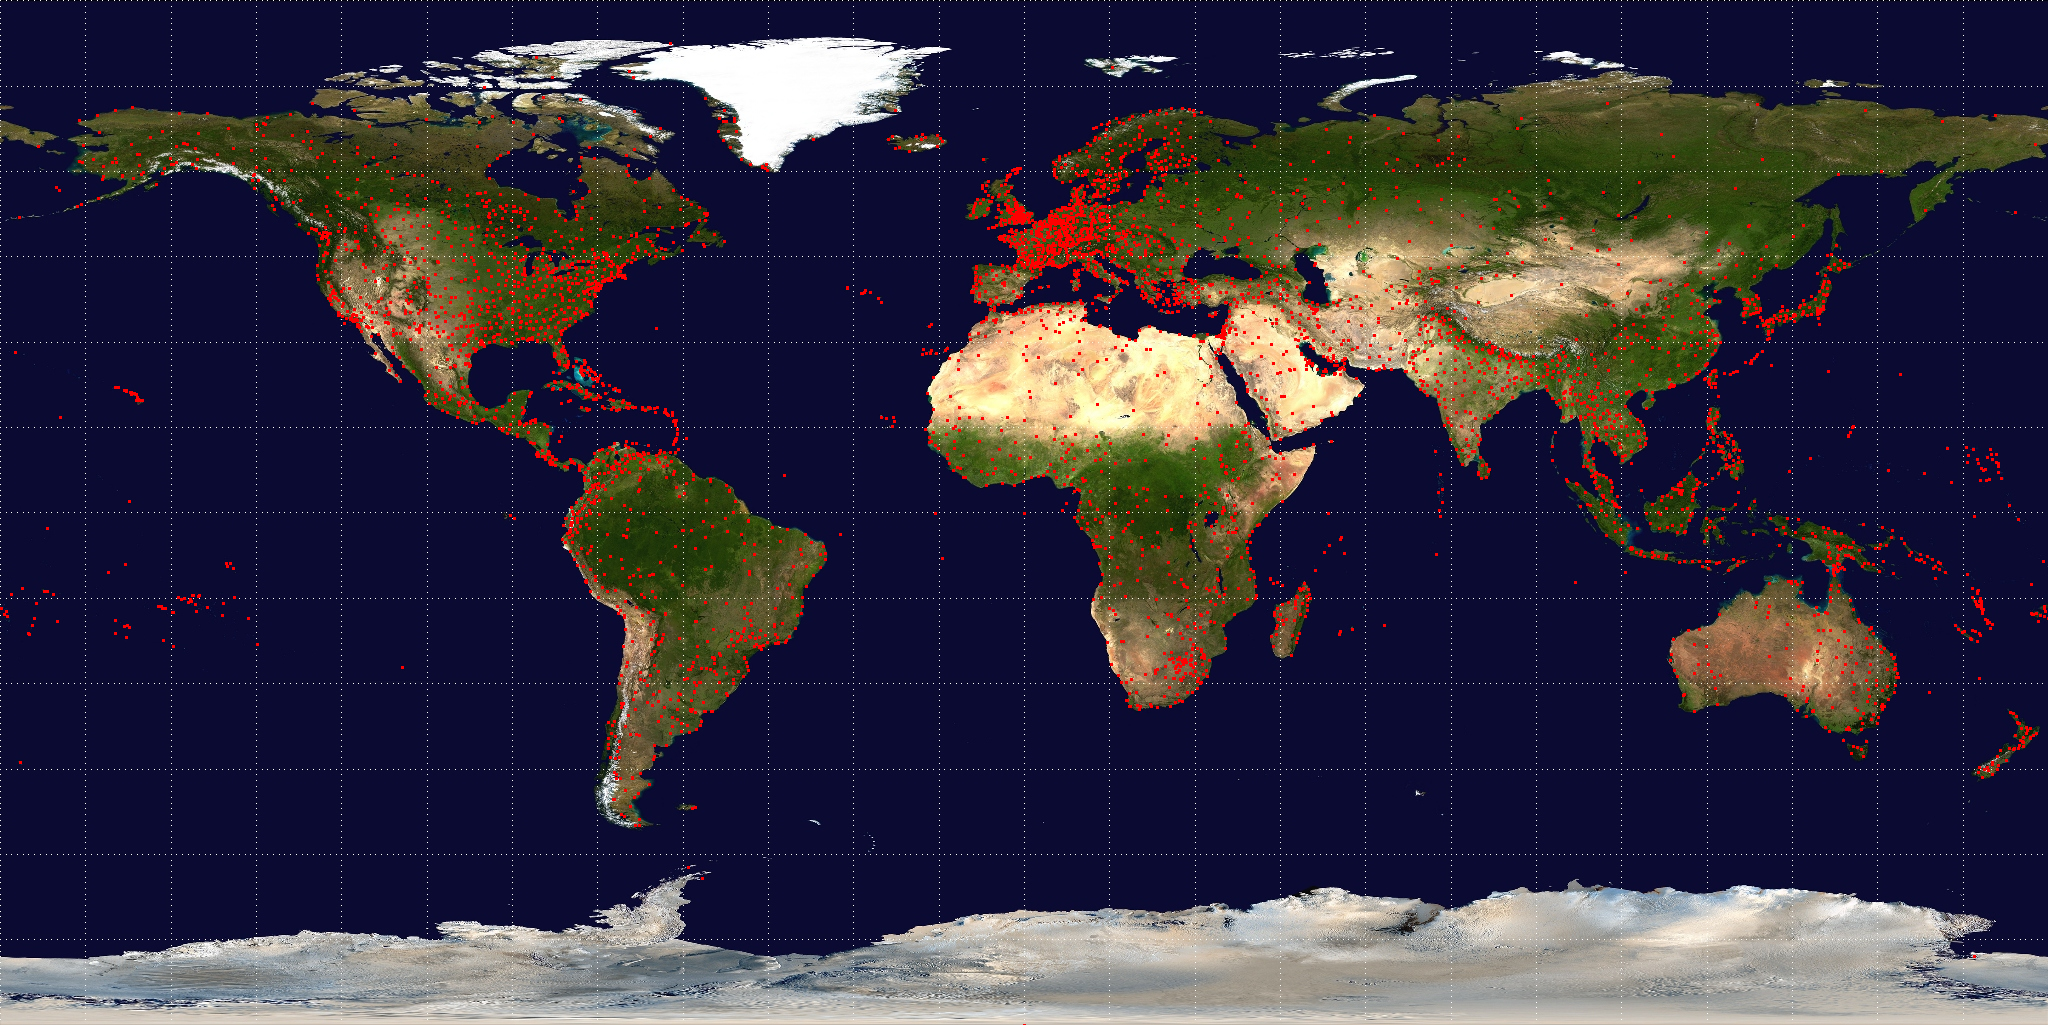
\includegraphics[width=\linewidth]{openflights-apdb-2048.png}
\end{figure}
\newpage
\section{Introduction}
In this lab we want to compute the page rank of airports using the network defined by routes from and to airports. For that, we used the supplied data downloaded from  \href{https://openflights.org/data.html}{\textit{Open flights}}\footnote{More details about the data structure can be found in the lab:  \href{http://www.cs.upc.edu/~ir-miri/labs/session3.zip}{Session03}}:
\begin{itemize}
    \itemsep-0.5em 
    \item {\fontfamily{qcr}\selectfont airport.txt} - contains a list of airports (nodes) from the world.
    \item {\fontfamily{qcr}\selectfont routes.txt} - contains a list of routes (edges) from the world.
\end{itemize}
As explained in the lab, we can represent this information as a graph, where airports are nodes and routes are edges. The weights of the edges will be the number of flights between two airports. Airports with high PageRank value are \textit{important} airports. This is crucial information when designing and reforming airport as it means that many flights (with passengers and goods) pass it. Optimizing the operation of such airport, will lead to improvement of many supply chains and other visitors.

\section{Implementation Scheme}
\subsection{Data Structures}
While analyzing {\fontfamily{qcr}\selectfont airport.txt} we found $7,663$ airport records. $1,923$ of them don't have IATA code, $2$ of them appear twice which leave us with $5,738$ "valid" airports. Representing the problem in two-dimensional array (matrix) will consume $~2^{25}\times sizeof(datatype)$ bytes. Since the max weight is $534$ (ORD - Chicago Ohare Intl, United States) our datatype must be at least 2-bytes, i.e. total of 64 Mega-Bytes. Since the matrix is very sparse, in order to save data space\footnote{In fact, 64MB it is not too big, It might be better to save the data as matrix in order to save data manipulation.}, we decides to save the information in two dictionaries, one for each, airport and routes (see figure.\ref{fig:uml}) 
\begin{figure}[h]
    \centering
    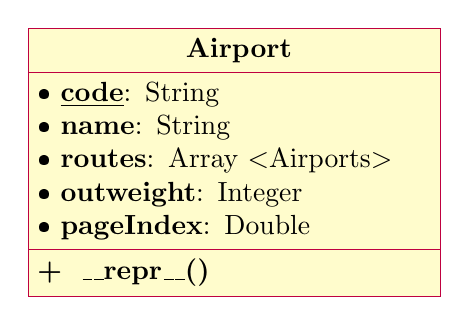
\begin{tikzpicture}
    \begin{class}[text width = 5cm]{ Airport }{0 ,0}
        \attribute {\textbullet \  \textbf{\underline{code}}: String}
        \attribute {\textbullet \ \textbf{name}: String}
        \attribute {\textbullet \ \textbf{routes}: Array \textless Airports\textgreater}
        \attribute {\textbullet \ \textbf{outweight}: Integer}
        \attribute {\textbullet \ \textbf{pageIndex}: Double}
        \operation {\textbf{+ \ \_\_repr\_\_()} }
    \end{class}
    \end{tikzpicture}

    \hspace{5pt}

    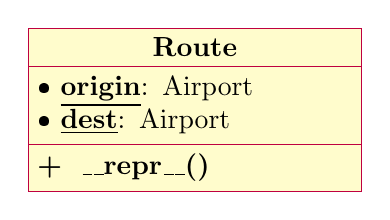
\begin{tikzpicture}
    \begin{class}[text width = 4cm]{Route}{0 ,0}
        \attribute {\textbullet \  \textbf{\underline{origin}}: Airport }
        \attribute {\textbullet \  \textbf{\underline{dest}}: Airport }
        \operation {\textbf{+ \ \_\_repr\_\_()} }
    \end{class}
    \end{tikzpicture}

\caption{Class diagrams}
\label{fig:uml}

\end{figure}


\subsection{Difficulties and Choices}
\noindent\fbox{%
    \parbox{\textwidth}{%
        \textcolor{red}{Laura!! I tried here to answer this question from the lab:} Modify the pseudocode above to add the effect of these (virtual) edges efficiently: how many of them are there, and how much pagerank do they add in total to each vertex in particular?
    }%
}
Our main difficulty was dealing with the \textit{airports} without departures(formally, \textit{dangling nodes}). There are three accepted approaches for treating pages with no outgoing links\cite{pageRank}:
\begin{enumerate}
    \item Eliminate such pages from the graph (iteratively prune the graph until reaching a steady state).
    \item Consider such pages to link back to the pages that link to them.
    \item Consider such pages to link to all web pages (effectively making an exit out of them equivalent to a random jump).
\end{enumerate}
The first approach can lead to loss of information. consider the graph in figure[\ref{graph:s0}] that represent our network, we can see that we can lose information about airports. The second and third approaches are more robust and promise that we will not lose information, we decided to add link to all nodes \textcolor{red}{(TRUE??)}. However, we don't keep it on the data structure itself, we add it to the iterative computation of the page-rank, therefore we won't "pay" for $n^2$ new edges.
\usetikzlibrary{arrows, automata, positioning}
\begin{figure}[h!]
    \begin{minipage}{0.24\textwidth}
    \scalebox{0.7}{
    \begin{tikzpicture}[
            > = stealth, % arrow head style
            shorten > = 1pt, % don't touch arrow head to node
            auto,
            node distance = 2cm, % distance between nodes
            semithick % line style
        ]
    
        \tikzstyle{every state}=[
            draw = black,
            thick,
            fill = white,
            minimum size = 4mm
        ]
    
        \node[state] (TLV) {$TLV$};
        \node[state] (BCN) [right of=TLV] {$BCN$};
        \node[state] (KOA) [below  of=BCN] {$KOA$};
        \node[state] (SYD) [below of=TLV] {$SYD$};
        \path[->] (TLV) [] edge node { } (BCN);
        \path[->] (BCN) [] edge node { } (KOA);
        \path[->] (KOA) [] edge node { } (SYD);
    \node[above,font=\bfseries] at (current bounding box.north) {Initial state\\};
    \end{tikzpicture}}
    \end{minipage}
    \begin{minipage}{0.24\textwidth}
    \scalebox{0.7}{
    \begin{tikzpicture}[
            > = stealth, % arrow head style
            shorten > = 1pt, % don't touch arrow head to node
            auto,
            node distance = 2cm, % distance between nodes
            semithick % line style
        ]
    
        \tikzstyle{every state}=[
            draw = black,
            thick,
            fill = white,
            minimum size = 4mm
        ]
    
        \node[state] (TLV) {$TLV$};
        \node[state] (BCN) [right of=TLV] {$BCN$};
        \node[state] (KOA) [below  of=BCN] {$KOA$};
        
        \path[->] (TLV) [] edge node { } (BCN);
        \path[->] (BCN) [] edge node { } (KOA);
        \node[above,font=\bfseries] at (current bounding box.north) {1st iteration - remove SYD};
    \end{tikzpicture}
    }
    \vfill
    \end{minipage}
    \begin{minipage}{0.24\textwidth}
    \scalebox{0.7}{
    \begin{tikzpicture}[
            > = stealth, % arrow head style
            shorten > = 1pt, % don't touch arrow head to node
            auto,
            node distance = 2cm, % distance between nodes
            semithick % line style
        ]
    
        \tikzstyle{every state}=[
            draw = black,
            thick,
            fill = white,
            minimum size = 4mm
        ]
    
        \node[state] (TLV) {$TLV$};
        \node[state] (BCN) [right of=TLV] {$BCN$};
        
        \path[->] (TLV) [] edge node { } (BCN);
                \node[above,font=\bfseries] at (current bounding box.north) {2nd iteration - remove KOA};
    \end{tikzpicture}}
    \end{minipage}
    \begin{minipage}{0.24\textwidth}
    \scalebox{0.7}{
    \begin{tikzpicture}[
            > = stealth, % arrow head style
            shorten > = 1pt, % don't touch arrow head to node
            auto,
            node distance = 2cm, % distance between nodes
            semithick % line style
        ]
    
        \tikzstyle{every state}=[
            draw = black,
            thick,
            fill = white,
            minimum size = 4mm
        ]
        \node[state] (TLV) {$TLV$};
        \node[above,font=\bfseries] at (current bounding box.north) {3rd iteration - remove BCN};
    \end{tikzpicture}
    }
    \end{minipage}
    \caption{1st approach}
    \label{graph:s0}
\end{figure}




\section{Experiments and Observations}
different dumping factors
about the converges parameter
other?


\newpage
\nocite{*}
\bibliographystyle{unsrt}
\bibliography{references}
\end{document}
